%%% Copyright (C) 2004 Claire M. Connelly and 
%%% the Department of Mathematics, Harvey Mudd College.
%%%
%%% This file is part of the sample thesis document provided to HMC
%%% mathematics students.
%%%
%%% See the COPYING document, which should accompany this
%%% distribution, for information about distribution and modification
%%% of the document and its components.

\chapter{Extracting Insights From Text Data}%
\label{sec:figs-and-tabs}

Topic modeling is an unsupervised learning algorithm that takes in a large corpus of text data and returns a specified number of representative topics found in the corpus. A topic is defined as probability distribution over fixed vocabulary. Words in a topic are sorted in descending order using the probability assigned to each word in the topic. The top $k$ words in a topic (for some $k$ defined by the user) reflect the overarching and related concepts of the topic. Topic modeling therefore provides a method of extracting insights about the high level meaning of a text. 
An example of an output of topic modeling is shown in figure \ref{fig:distribution}.
\begin{figure}[H]
    \centering
    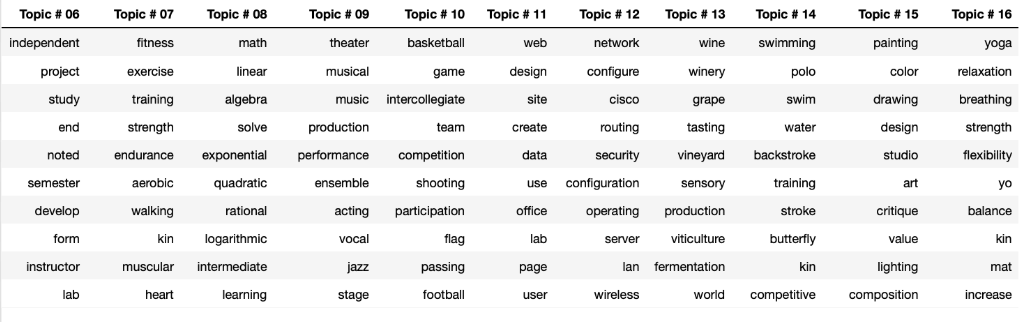
\includegraphics[scale=0.35]{topic-distribution.png}
    \caption{Example distribution of topics output by a trained topic model}
    \label{fig:distribution}
\end{figure}

\section{Methods}
Our team considered and explored two well-known methods for topic modeling:
    \begin{itemize}
        \item Latent Dirichlet Allocation, commonly known as LDA, is a generative probabilistic model that prescribes each document in a corpus with a finite mixture of topics from an underlying topic distribution. LDA views each document in a corpus as a generated item from a collection in order to infer the topic distribution. The generative process that LDA uses to infer the underlying topic distribution represents the topic distribution $\theta_m$ for each document $m$ as a random variable from a Dirichlet distribution with sparse priors, where each topic is a distribution over all of the words. For each of $N$ words in document $m$, a topic $z_n \sim \text{Multinomial}(\theta)$ is chosen and a word $w_n$ is chosen from a multinomial distribution conditioned on $z_n$. LDA requires the modeler to input number of topics. In our experiments, we built our LDA models from LdaModel in the gensim package. 

        \item Non-negative Matrix Factorization (NMF for short) takes in a bag-of-words $n\times m$ matrix $A$ whose entry $A_{ij}$ is the number of occurrences of word $j$ in document $i$. NMF seeks to find the closest approximation of $A$ as a product of a $n\times k$ matrix $W$ and a $k\times m$ matrix $H$ with the condition that all entries of $W$ and $H$ are non-negative. In other words, NMF outputs $W,H$ with the prescribed dimensions such that $\|A-WH\|_F$ is minimized.
        
        To interpret the output matrices $W$ and $H$, we call $W$ the \textit{basis matrix} and $H$ the \textit{coefficient matrix}. The prescribed number $k$ here represents the number of topics we wish to extract from the text. To find out the top words are associated with the $i$-th topic, we examine the $i$-th row of the $H$ matrix and take the words whose position in that row has a high value. In other words, the entry $H_{ij}$ measures how relevant word $j$ is for topic $i$. Next, if we want to find out what topics are the most prevalent in the $i$-th corpus document, we examine the $i$-th row of the $W$ matrix and take the topics whose position in that row has a high value. Although there are methods to perform this task with unseen documents that were not used in training, we omit their discussions here as they were not used for our experiments.
    \end{itemize}
In a later section, we discuss our preferred method and our reasons for choosing it.

\section{Assessing Insights}
\subsection{Topic Coherence}
Topic coherence is a standard method of comparing topic models. It measures how semantically cohesive each topic is. For example, we'd say that a topic that contained all medically-related words ("doctor," "stethoscope," "surgery," etc.) has a high coherence while a topic composed of unrelated words ("city", "toothpaste", "kittens") has low coherence. Our measure of coherence is the average pairwise similarity between the GloVe vector representations of the top three words of a given topic. 


By analyzing the mean topic coherence of a model compared to the number of topics in the model, we can determine the optimal number of topics for our model. As seen in figure \ref{fig:topic-coh}, topic coherence peaks where the model only has two topics. However, the team judged this to be an under-fit of the model. In this case, the optimal number of topics chosen was 16, the next highest peak. 
\begin{figure}[H]
    \centering
    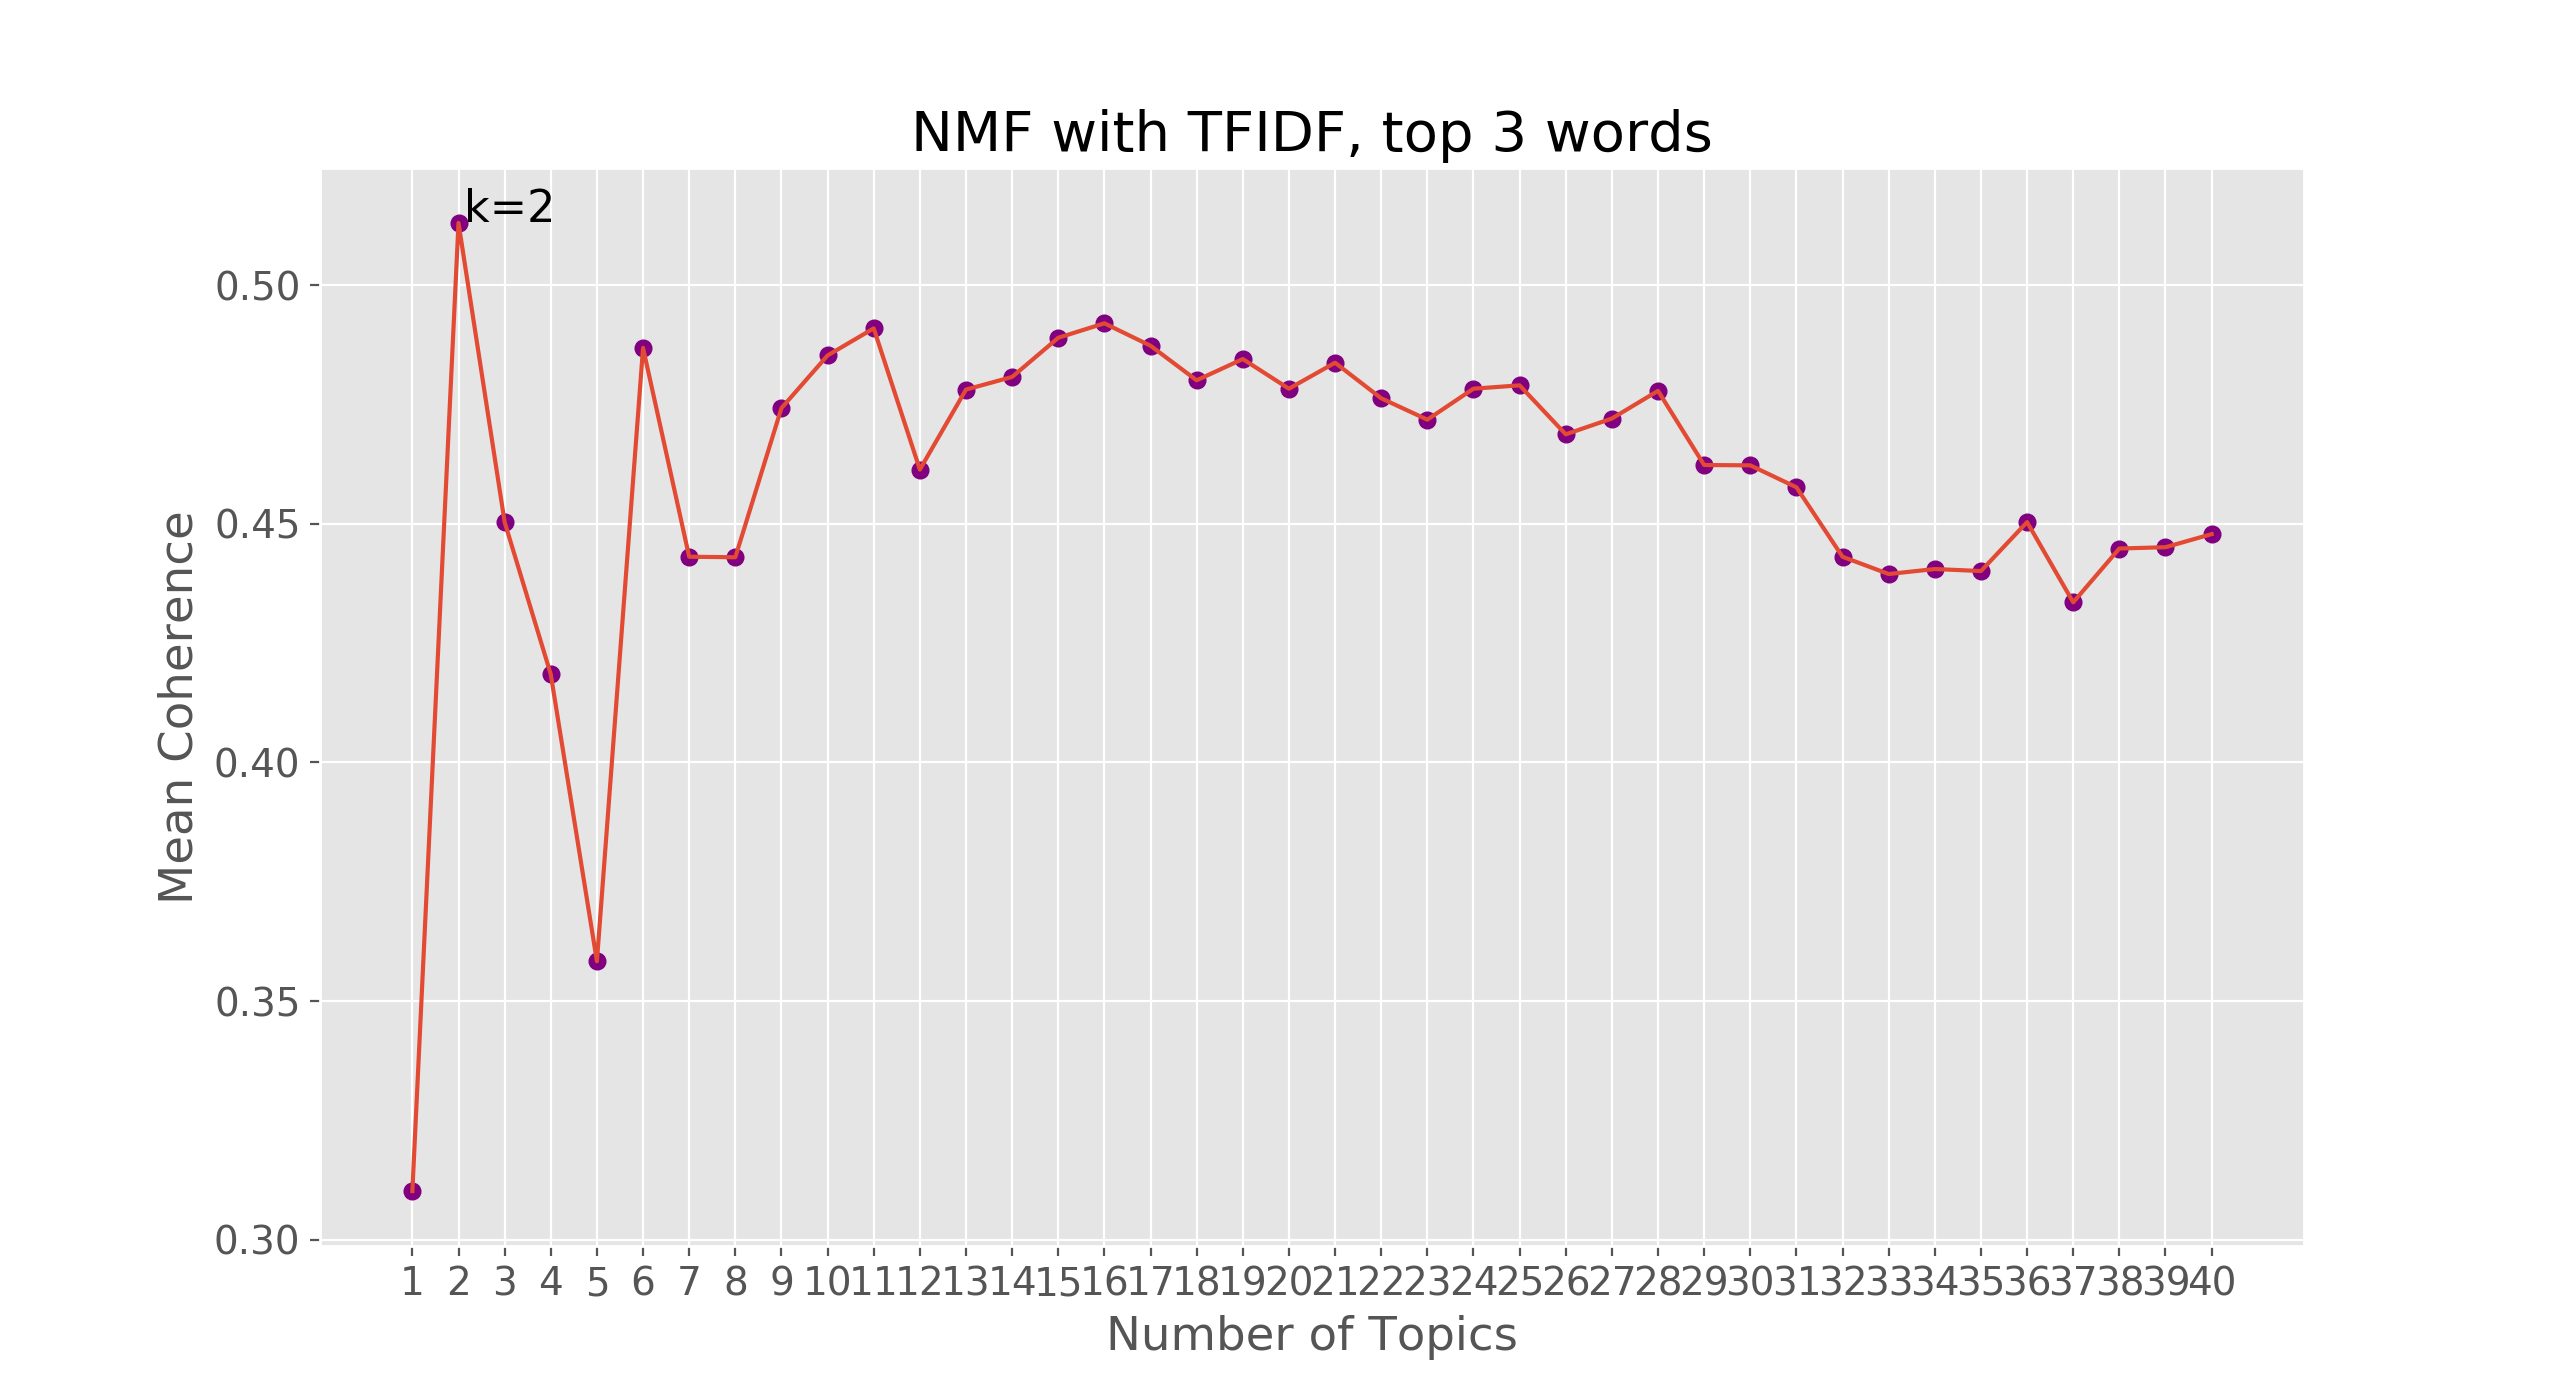
\includegraphics[scale=0.15]{topiccoh.png}
    \caption{Topic Coherence vs Number of topics using the first 3 words of every topic}
    \label{fig:topic-coh}
\end{figure}

\section{LDA vs NMF}
We ran experiments to determine which topic modeling technique would perform well for our purposes, specifically on Los Positas Syllabi. We trained models using both techniques and graphed the mean topic coherence of the outputs from the models to judge which technique performed better. From the graph in figure \ref{fig:lda_vs_nmf}, we see that for the range of number of topics considered, NMF consistently had higher mean topic coherence than LDA, and hence chose it for our model and the rest of our analysis. This was expected since NMF is said to perform better on sparser and smaller data sets (Chen, Zhang, Liu, Ye, \& Lin, 2019). However, we did provide flexibility in the module so that the modeler could use an LDA model if they prefer. 
\begin{figure}[H]
    \centering
    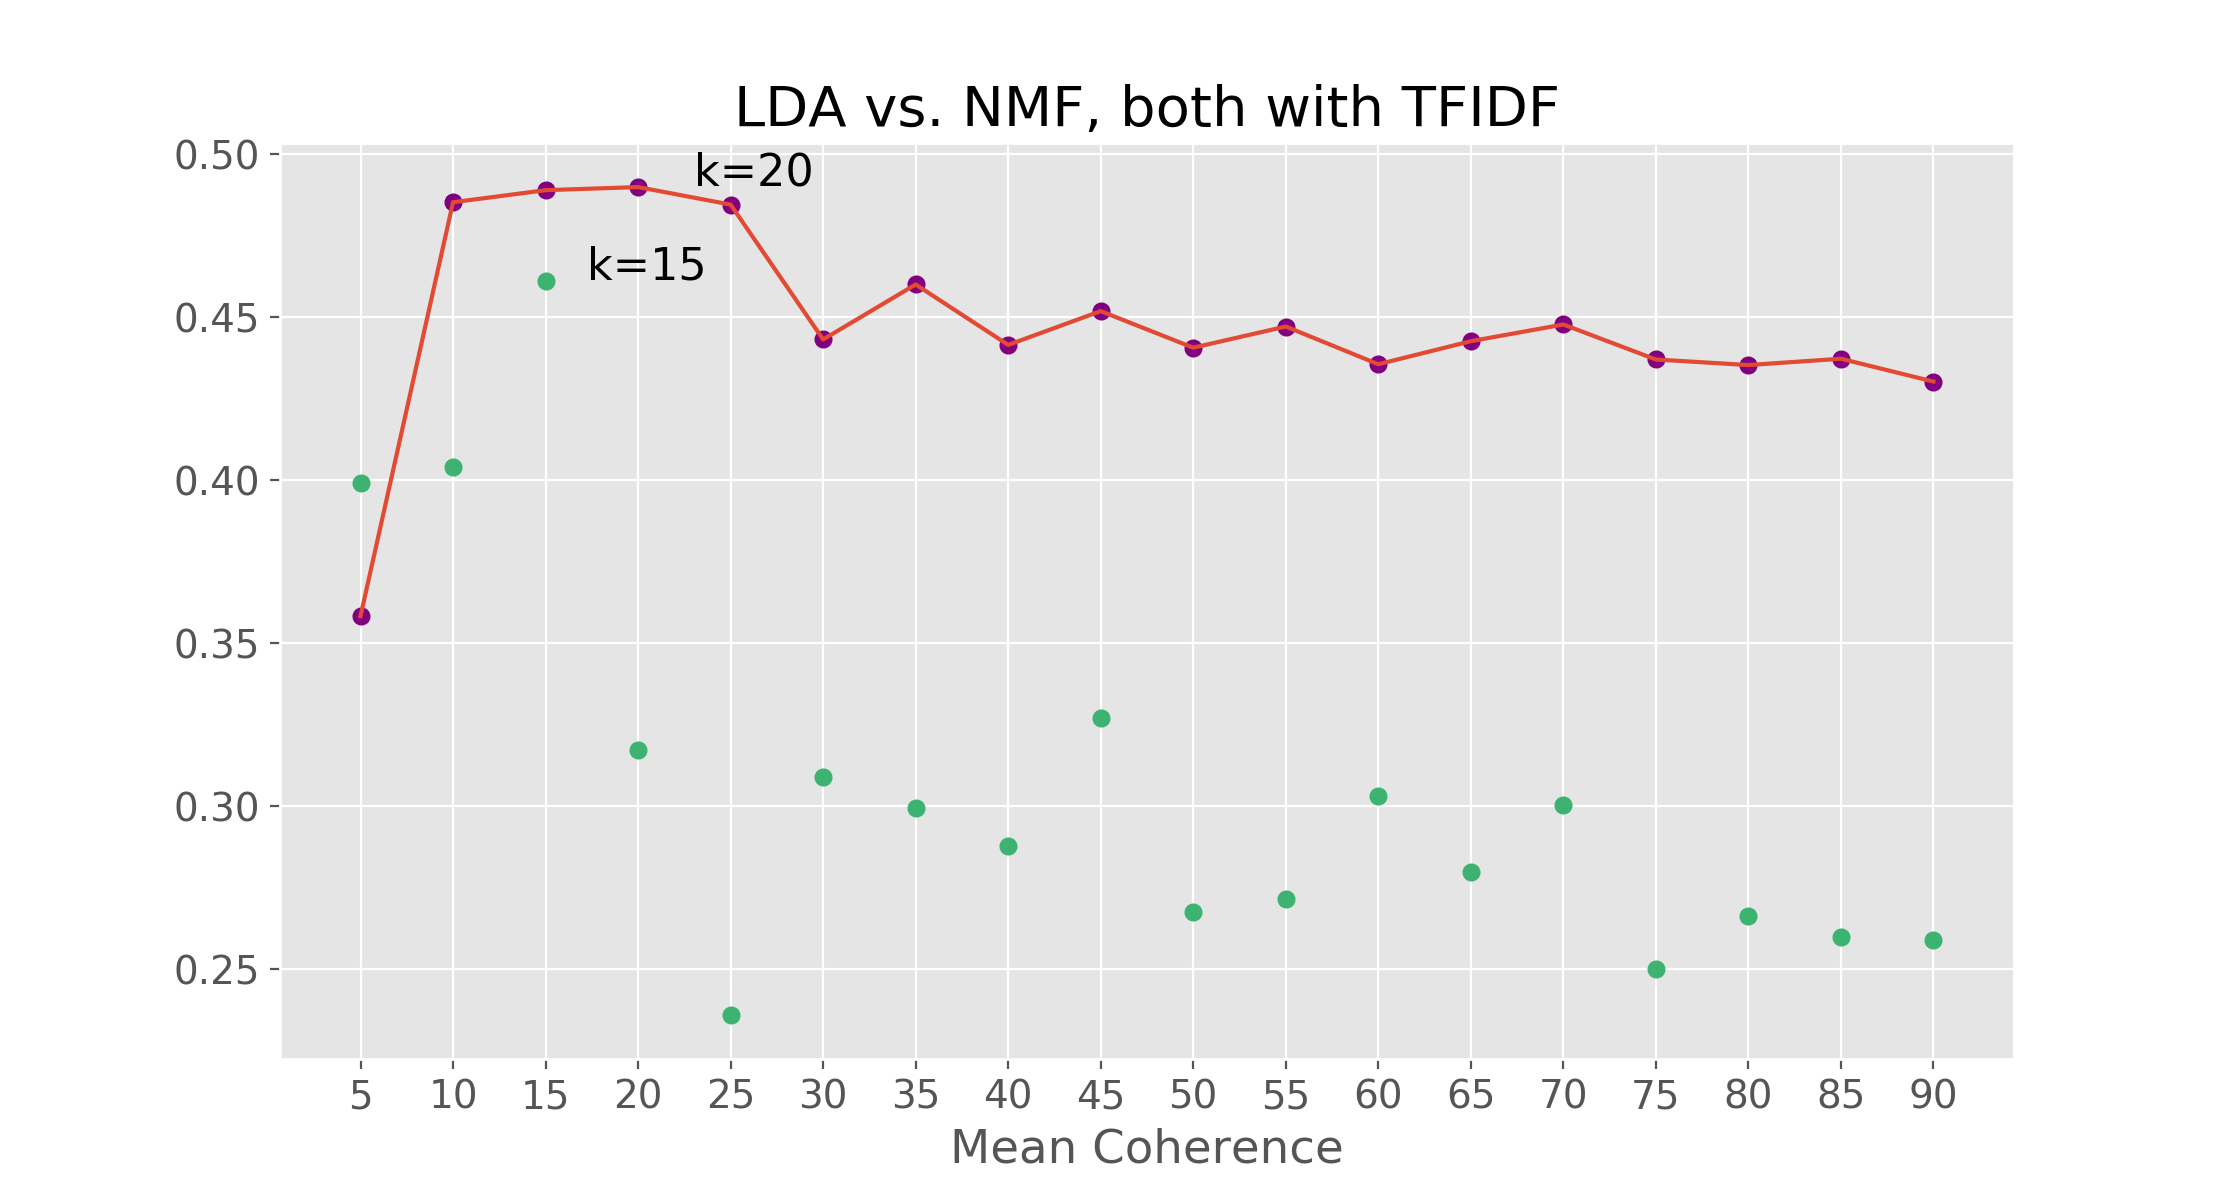
\includegraphics[scale=0.15]{LDAvsNMF.png}
    \caption{Topic Coherence of LDA compared to NMF. Models with NMF are shown with the line graph, and LDA are shown with dots}
    \label{fig:lda_vs_nmf}
\end{figure}

\section{Extracting insights}
Our goal is to leverage topic modeling to visualize high level themes represented in a corpus containing all the syllabi of an educational institution. By doing so, we can estimate the emphasis of each topic in the curriculum of the institution, as well as the overall educational priorities of the institution.

\subsection{Data}
Our dataset consists of 2,841 syllabi from Las Positas Community College in Livermore, California, which we obtained by scraping course syllabi publicly available on their \href{http://www.curricunet.com/laspositas/search/course/course_search_result.cfm}{website}.
\url{http://www.curricunet.com/laspositas/search/course/course_search_result.cfm}

\subsection{Visualization of Results}
The output of our trained NMF topic model is shown in figure \ref{fig:nmf-viz}. Each dot in this figure represents the 2D vector representation of a syllabus in the corpus. The color of these dots are determined by the topic they relate the most to. The top 3 words in each topic are printed alongside the syllabi-dots that are most related to it. Also, inter-dot distance is a measure of how similar the two syllabi are. 
\begin{figure}[H]
    \centering
    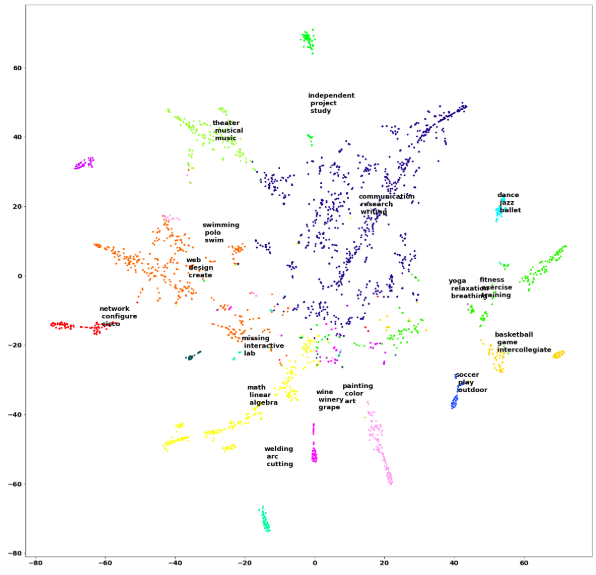
\includegraphics[scale=0.5]{nmf-visualization.png}
    \caption{Visualization of NMF results of Las Positas data. Here we see that the topic related to communication, research and writing is prevalent across many syllabi in the corpus. These syllabi-dots are also spread out, implying that the syllabi related to this topic are similar to other syllabi in the corpus as well. In contrast, the topic related to dance, jazz, and ballet is less prevalent, and is dominant in syllabi that are only similar to other syllabi within the same topic.}
    \label{fig:nmf-viz}
\end{figure}


\subsection{PilotCity Deliverable}

Our deliverable is a fully-functioning topic modeling package for PilotCity's use. The structure of our module is seen in figure \ref{fig:pipeline}. 
\begin{figure}[H]
    \centering
    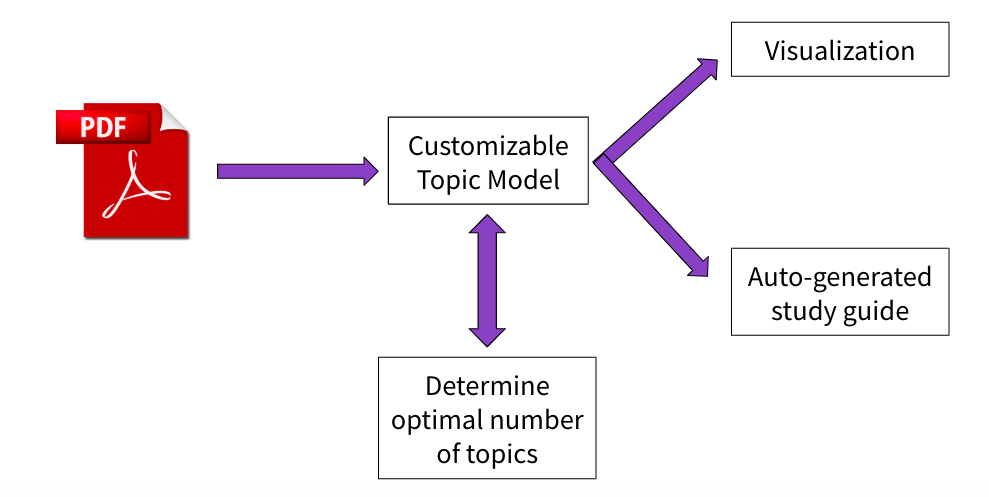
\includegraphics[scale=0.35]{module-pipeline.png}
    \caption{Pipeline for topic modeling module}
    \label{fig:pipeline}
\end{figure}
The module takes a folder of PDFs as input and cleans and tokenizes the text in each document. It also filters out the most common words across all documents using an algorithm called 'term frequency inverse data frequency', or TFIDF. These cleaned documents are used to train an NMF topic model, where the optimal number of topics is programmatically determined based on topic coherence. The model is saved, and visualized as in figure \ref{fig:nmf-viz}. 
Given an unseen syllabus and a trained topic model, our module can also extract the most representative topics from the syllabus and search Wikipedia for word definitions to automatically generate a study guide prototype. An example of an auto-generated study-guide is seen in figure \ref{fig:studyguide}.
We delivered the module to the PilotCity team and lead a training session to help them understand the potential use cases for the module during our spring site visit. 
\begin{figure}[H]
    \centering
    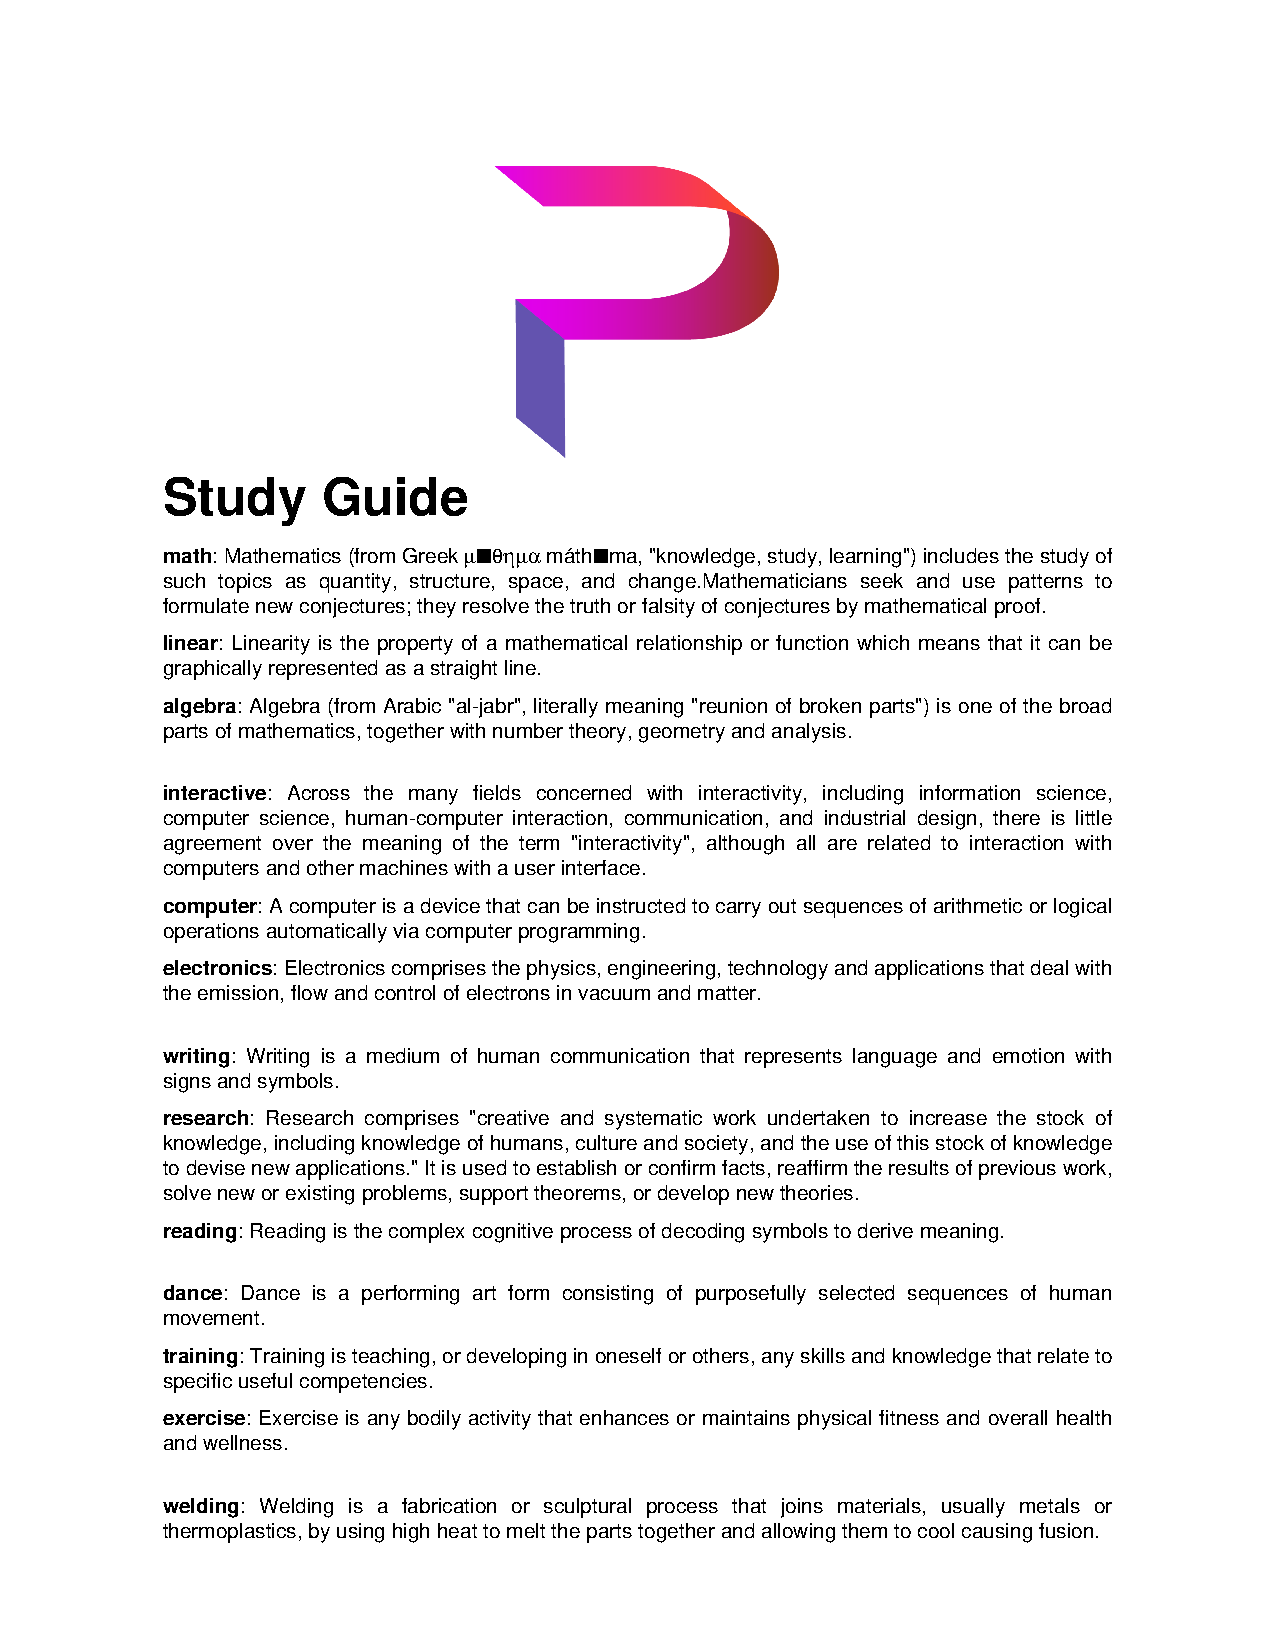
\includegraphics[scale = 0.5]{studyGuide_youJustMade.pdf}
    \caption{Auto-generated study guide}
    \label{fig:studyguide}
\end{figure}

\section{Further work with Topic Modeling}
In addition to running our topic model on syllabi of an institution to gauge current educational priorities, we also ran our topic model on syllabi of classes taught across many years to judge the change of an institution's educational priorities over time. This application is discussed further in the paper attached. 




